%%% Custom Commands

\newcommand{\Z}{\mathbb{Z}}
\newcommand{\abar}{\overline{a}}
\usepackage{tikz,enumitem}
\usetikzlibrary {shapes.geometric}

%%

Consider the diamond as follows. (For clarity: all edges and the horizontal diagonal of length 1.)

	\begin{center}
		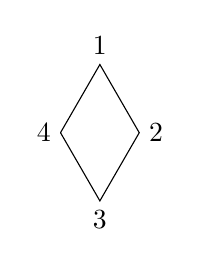
\begin{tikzpicture}
			\setlength{\unitlength}{1in}
			\draw (0,0) -- (.5,.866) -- (1,0) -- (.5,-.866) -- (0,0) node[anchor=east] {4} (.5,.866) node[anchor=south] {1} (1,0) node[anchor=west]{2} (.5,-.866) node[anchor=north] {3};
		\end{tikzpicture}
	\end{center}
	
	\begin{enumerate}[label=(\alph*)]
		\item Using $r$ as rotation by $90^\circ$ and $f$ as a flip along the vertical axis at the center of this figure, as in $D_4$, write all of the symmetries of this diamond in terms of $r$ and $f$.  That is, which combinations of $r$ and $f$ return this shape to the same location, possibly with the numbers swapping?
		\vskip 2in
		\item Write and complete a Cayley table for the group you found in part (a).
		\vfill 
		\item What group ($\Z_n$, $\Z_m\times\Z_n$, $S_n$, $D_n$, $\dots$) is this group of symmetries isomorphic to? Specifically you should be considering the following questions: What is the order of the group? Is this group cyclic? If it is not cyclic is it at least abelian?
		\vskip 1in
	\end{enumerate}
	
%%

Consider the square as follows. (For clarity: the double-marked edges of the square shown are painted blue. And for the shape to remain the same, the blue edges must remain blue.)

	\begin{center}
			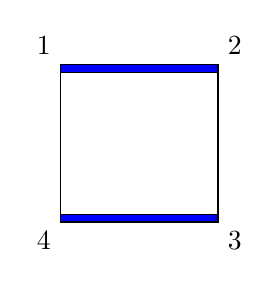
\begin{tikzpicture}
				\draw (0,0) rectangle (2,2) node[anchor=south west] {2} (2,0) node[anchor=north west] {3} (0,0) node[anchor=north east] {4} (0,2) node[anchor=south east] {1};
				\draw[fill=blue] (0,.1) rectangle (2,0);
				\draw[fill=blue] (0,1.9) rectangle (2,2);
			\end{tikzpicture}
	\end{center}
	
	\begin{enumerate}[label=(\alph*)]
		\item Using $r$ as rotation by $90^\circ$ and $f$ as a flip along the vertical axis at the center of this figure, as in $D_4$, write all of the symmetries of this square in terms of $r$ and $f$.  That is, which combinations of $r$ and $f$ return this shape to the same location, possibly with the numbers swapping?
		\vskip 2in
		\item Write and complete a Cayley table for the group you found in part (a).
		\vfill 
		\item What group ($\Z_n$, $\Z_m\times\Z_n$, $S_n$, $D_n$, $\dots$) is this group of symmetries isomorphic to? Specifically you should be considering the following questions: What is the order of the group? Is this group cyclic? If it is not cyclic is it at least abelian?
		\vskip 1in
	\end{enumerate}

%%

Consider the dart as follows. (For clarity: this is an isocoles triangle with a bend in the middle of the bottom.)

	\begin{center}
		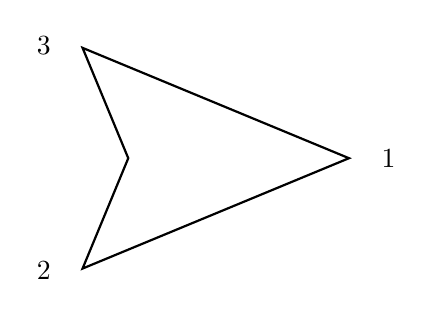
\begin{tikzpicture}
			\setlength{\unitlength}{1in}
			   \node[dart, draw, black, thick, inner sep=.25in]			(d) {};
			   \node [right=.1in] at (d.tip) {1};
			   \node [left=.1in] at (d.right tail) {2};
			   \node [left=.1in] at (d.left tail) {3};
		\end{tikzpicture}
	\end{center}
	
	\begin{enumerate}[label=(\alph*)]
		\item Tell me what you mean by $r$ and $f$ when finding the symmetry group of this shape, and tell me what the symmetry group is.
		\vskip 2in
		\item Write and complete a Cayley table for the group you found in part (a).
		\vfill 
		\item What group ($\Z_n$, $\Z_m\times\Z_n$, $S_n$, $D_n$, $\dots$) is this group of symmetries isomorphic to? Specifically you should be considering the following questions: What is the order of the group? Is this group cyclic? If it is not cyclic is it at least abelian?
		\vskip 1in
	\end{enumerate}